\chapter{Measurement technique}
\section{Heating}
\label{sec:heating}
%This section will be devoted to the following topics:
%\begin{enumerate}
%	\item The circuit design to achieve mK level broadening in the thermal reservoir while preventing any potential from developing in the reservoir, which would effectively shift the chemical potential of the reservoir.
%	\item Techniques used to apply synchronously apply two, 90$^{\circ}$ out of phase square wave heating signals on either side of a remote quantum point contact, allowing for heating in separate bath while preventing a monopole electric moment from affecting the entropy measurement.
%\end{enumerate}

The measurement protocol as laid out in Ch.~\ref{ch:Methods} requires the ability to vary the temperature of the system. It was mentioned that this is completed by directly (Joule) heating the electrons in a reservoir coupled to the quantum dot, however the mechanism of this heating was not discussed in depth. In practice, there are a number of limitations that must be considered when constructing a strategy to induce the $\delta T$ oscillations necessary for entropic measurements as they were completed in this thesis. 

The first, and most important, of these limitations is that frequency of the heating, $f_{heat}$, must be sufficiently large that charge noise in the quantum dot and charge sensor do not affect our determination of $dN/dT$. Our measurements utilize a continuous measurement of $dN/dT$ as function of chemical potential (see Sec.~\ref{sec:data_analysis}) however the detrimental affects of a too small $f_{heat}$ can also be understood in the context of repeated measurements of the transition at varying temperatures. If $f_{heat}$ is small, then the `period' of these measurements -- time between successive measurements of the transition at different temperatures -- will be large. Charge noise in the quantum dot can be thought of as a poisson process and therefore goes as $1/f$~\cite{fujisawa2000charge}. This means that the larger the time between successive measurements, the more likely a charge jump will occur. Because the protocol relies on the small relative shift between occupation curves at different temperatures, it is exceedingly sensitive to disturbances in the occupation of the quantum dot between measurements. Effectively, this precludes any heating not localized on the device as it will take too long to equilibrate through the entirety of whatever larger system is being heated. 

One way to accomplish localized heating is by directly heating the electrons in the \ac{2DEG} using Joule (resistive) heating. It has been shown that, at sufficiently low temperatures, resistive heating can be used to locally raise the temperature of an electron reservoir~\cite{mittal1996electron}. Furthermore, in Hartman et al.'s previous work in the group, it was showed that a version of Joule heating worked to effectively heat an electron reservoir and measure entropy. Electrons are heated through a \ac{QPC} into a narrow channel from a distance of about 5 $\mu$m from the quantum dot. This heat can quickly thermalize with cold ground ohmic contacts to the channel at either end, but while a current is applied, the temperature of the reservoir can be locally controlled. However, this technique leads to the second difficulty which is that the heating of the reservoir (tunnel) coupled to the quantum dot must \textit{only} change its temperature, and not also change its chemical potential. If the chemical potential of the reservoir is also increased/decreased while heating, it will appear like a relative shift in the center of the transition in the quantum dot. For sufficiently small current biases across this \ac{QPC}, very little potential builds, and so the `pure' thermal broadening approximation is valid. However, in the limit of larger current bias, or small $dN/dT$ signal (with respect to this small shift from a change in chemical potential), this technique breaks down. The final complication is that not only can potential in the reservoir coupled to the dot affect the center of transition, but a sufficiently large potential in a nearby reservoir can also induce shifts to the center of the transition. This can most easily be understood as an effective electrostatic gating. 

In Fig.~\ref{fig:fulldevice}, the full schematic for the device used in this thesis is presented. At its most simple level, this represents a two-stage variation of the version outlined in the previous paragraph. In the first stage, electrons are heated by opposing currents through the pair of heating QPCs. By applying an exactly antisymmetric square wave current signal, the affect on the quantum dot of potential in these reservoirs is kept to a dipole moment. Because small potentials will still develop in this first stage, a constriction in the form of another \ac{QPC}, the `source', is defined between this first stage at $T_{hot}$ and the next stage, at $T_{mid}$. It is tuned to about 12 k$\Omega$, or in the language of the \ac{QPC}s, the first plateau\footnote{This is a plateau at conductance equal to $2e^2/h$. Conductance is quantized in the ballistic regime through a narrow constriction. The thermal conductivity through \ac{QPC}s is well studied, a nice summary of the subject can be found here~\cite{van2005quantum}.}.
\begin{figure}[h]
\centering
\resizebox{1\textwidth}{!}{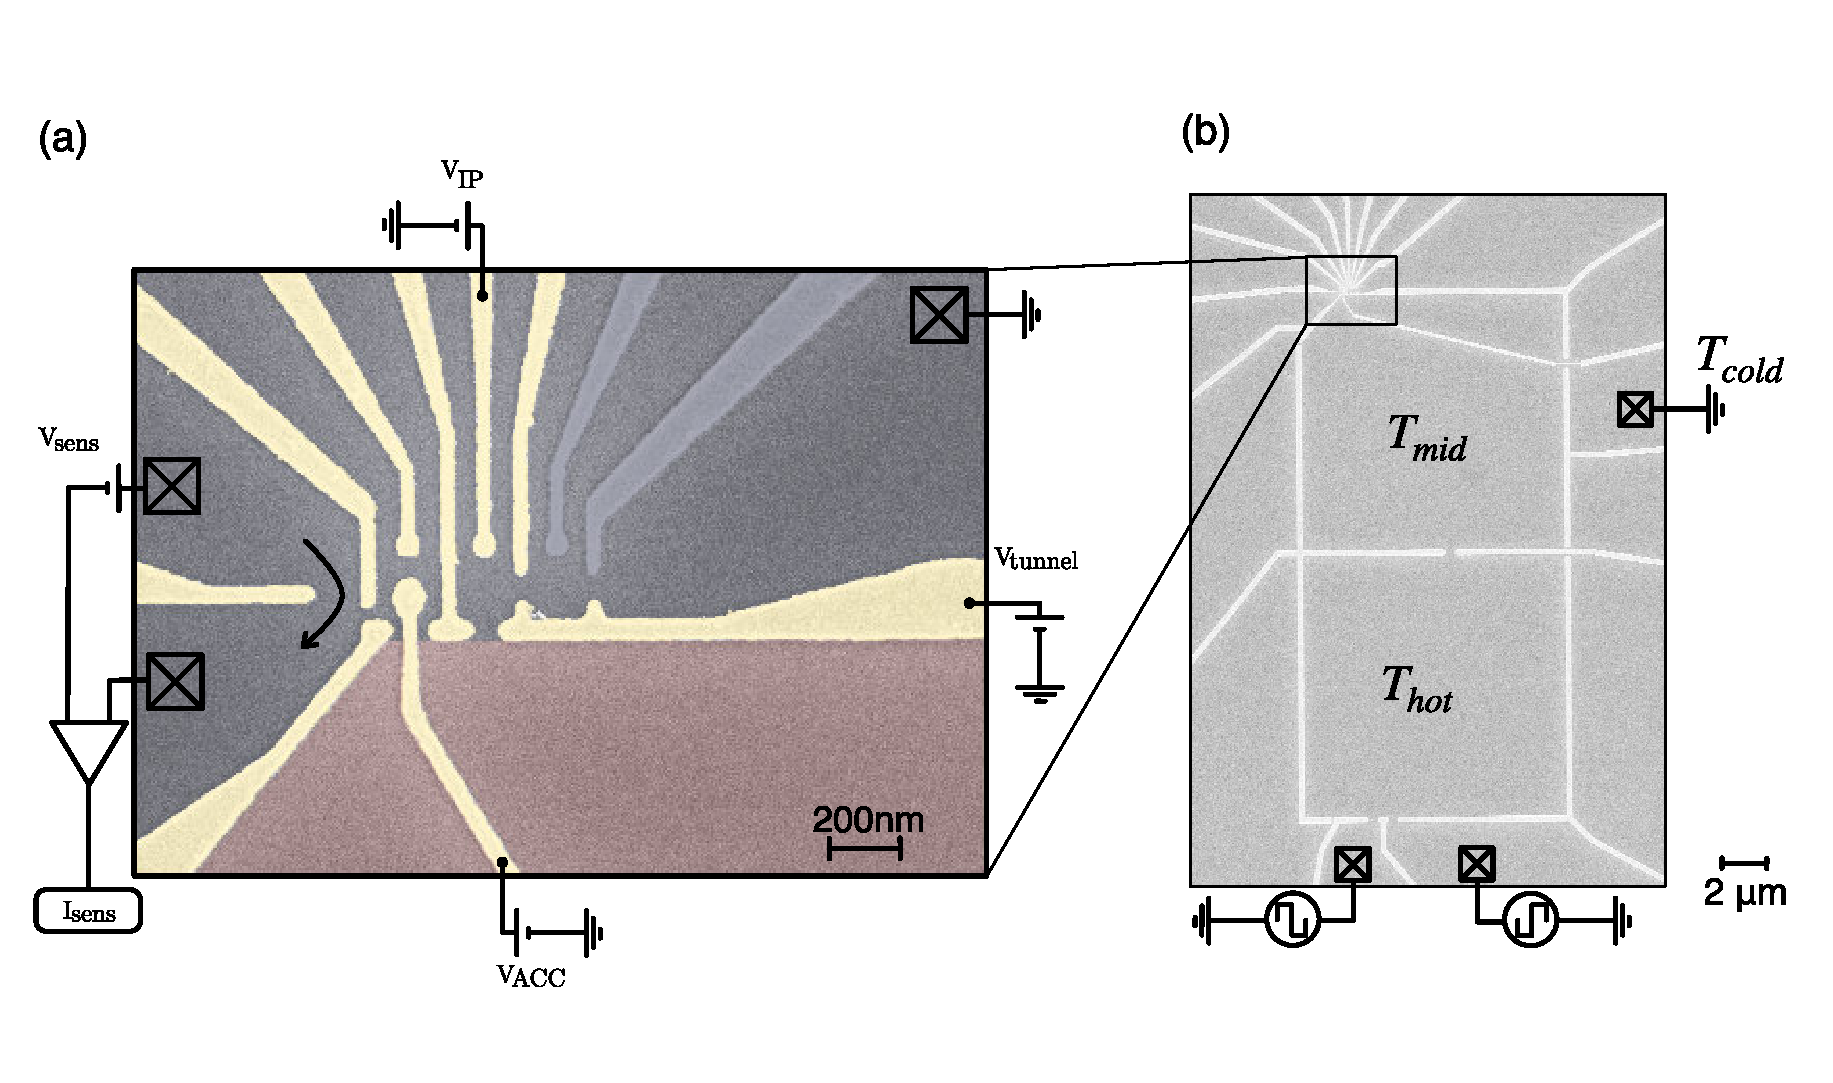
\includegraphics{figures/pdfs/all_parts_device.eps}}
\caption{In (a) the double dot system from measurements in this thesis is shown on a top-down false-color \ac{SEM} image. In (b) the relation of this device to the other components of the heating apparatus are shown on another top-down \ac{SEM} image. The two stage heating is labelled by $T_{hot}$: stage 1, then $T_{mid}$: stage 2. A number of \ac{QPC}s control the connection between these stages including the HQPCs which are used for heating, the SQPC which is the source of heat for the second stage, and the DQPC which is the drain for the second stage.}
\label{fig:fulldevice}       
\end{figure}
Small thermocurrents through this constriction allow the second reservoir to heat up in response to changes in temperature in the first without inducing non-neglible potentials in the reservoir coupled to the quantum dot. Finally, a `drain' \ac{QPC} is used to allow the electrons in the second reservoir to thermalize with a large cold bath of electrons labelled $T_{cold}$ when the heater bias is turned off and the `source' stops supplying heated electrons. In practice, this scheme allows for measurements of entropy in our system while heating with a $\delta T$ up to a few 100 mK from our base temperature which is usually $\leq 100$ mK. Limitations in heating further come from the electron-phonon dissipation of the heating power which strengthens as $T$ is increased.


\section{Extraction of dN/dT signal}
\label{sec:data_analysis}
This section will be devoted to the following topics:
\begin{enumerate}
	\item The techniques used to allow for repeated measurements and used to fit and extract entropy signals.
\end{enumerate}


\section{Artifacts from cross couplings}
\label{sec:artifacts}

\begin{figure}[h]
\centering
\resizebox{1\textwidth}{!}{\includegraphics{figures/pdfs/dndt_artifact.eps}}
\caption{}
\label{fig:dndt_artifact}       
\end{figure}

\section{Back action noise}
\label{sec:back}


\section{Determination of electron temperature}
\label{sec:electrontemp}

In the past few sections and in Ch.~\ref{ch:Methods}, a great deal of attention was brought to temperature of the system and to oscillations, $\delta T$, to the temperature which allow for measurements of $dN/dT$ and subsequently, $\Delta S$. It was stated that the temperatures can be exactly determined by thermal broadening of the Fermi distribution in the reservoir, and in particular Eqn.~\ref{eqn:occupation} was referenced as a means of calculating the exact broadening of the Fermi distribution by the broadening of the lineshape of the occupation ($N(\mu)$) curve. In this section, this assumption is experimentally justified and an approximate base electron temperature is established. 

To start, consider an experimental form of Eqn.~\ref{eqn:occupation} to allow for direct fitting to data as it is collected -- $I_{sense}$ as a function of $V_{ACC}$~\cite{nikentropy}.
\begin{equation}
	\label{eqn:exp_isense}
	 I_{sense}(\Theta, V_{ACC}) = I_0 \tanh\left(\frac{V_{ACC} - V_{mid}(\Theta)}{2\Theta}\right) + \gamma \,\, V_{ACC} + I_1
\end{equation}

Where $I_0$ represents the amplitude of the transition in terms of current, $V_{mid}$ the center of the transition in terms of gate voltage, and $I_1$, the current at the center point of the transition. The (constant) $\gamma$ term allows for an effective linear cross capacitance between $V_{ACC}$ and the current through the charge sensor. In this context, $\Theta$ gives the thermal broadening of the transition in gate voltage. Importantly, $\Theta \propto k_B T$. 

In Fig.~\ref{fig:etemp}, the temperature of the \ac{MC} plate on which the sample is mounted is varied, and repeated measurements of the transition (two examples shown in (b)) are acquired. 
\begin{figure}[h]
\centering
\resizebox{1\textwidth}{!}{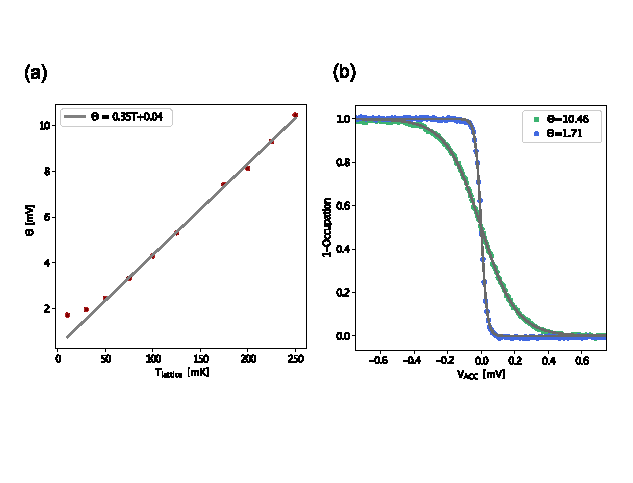
\includegraphics{figures/pdfs/electron_temp_panel.eps}}
\caption{By fitting the transition line shapes of the 0 $\to$ 1 electron transition in the quantum dot, one can extract the broadening of the fermi energy in the reservoir. By varying the lattice temperature of the substrate and plotting the effective broadening of the fermi sea ($\theta$) at each lattice temperature, we can extract the effective electron temperature, $T_e$. Here $T_{e, \, base} \approx 35$ mK.}
\label{fig:etemp}       
\end{figure}
Each is fit to Eqn.~\ref{eqn:exp_isense} yielding a value $\Theta$ in mV which is plot in Fig.~\ref{fig:etemp} (a). For the majority of the plot, as expected, the thermal broadening of the transition, represented by $\Theta$, goes like $T$. Therefore, in the linear regime, it is quite clear that any temperature oscillation $\delta T$ will be proportional to a $\delta \Theta$. 

It is useful to also consider the deviation in $\Theta$ away from this linear fit at very low $T$. This is a byproduct of a combination of radiation increasing the temperature of the electrons and weak electron-phonon coupling. It is a well known effect~\cite{PhysRevB.49.5942}, and thus the most experimentally important metric about any given cryogenic system operating at mK temperatures is the effective base electron temperature, and not the the base lattice temperature. The non-linearity in the $\Theta$ vs $T$ curve, then, is a result of this deviation between electron and lattice temperature, since $\Theta \propto k_B T_e$. By extrapolating the linear $\Theta (T)$ curve to smaller $\Theta$, we can conclude that the effective base $T_e$ is about 35mK at our base fridge temperature.

\chapter{Measurement setup}

To make the measurements in this thesis, a great deal of work was put into developing a low noise wiring solution for the low frequency DC measurements necessary for measuring entropy in our devices. Because of the work of many previous students, nearly all of the instrumentation used as well as power supplies for these instruments have already been heavily optimized. 

Specifically the instrumentation used was, for DC data acquisition as well gating the device, a modified openDACs DAC-ADC in conjunction with a Basel Precision Instruments current pre-amplifier.\footnote{Available at \url{http://opendacs.com} and \url{https://www.baspi.ch} respectively. Modified openDACs source code was developed by members of the lab, Tim Child and Christian Olsen, in conjunction with Mark Carlsen. Available at \url{https://github.com/folk-lab/FastDAC}} Both instruments are powered by a low noise isolation transformer paired with inverters. 

Measurements were completed in a dry dilution refrigerator -- Bluefors XLD Dilution Refrigerator. A well known problem with dry systems is that their use of a pulse tube cryocooler induces a large amount of vibrational noise. It is thought that these vibrations can induce electrical noise in the measurement lines due to a triboelectric mechanism~\cite{pelliccione2013design, kalra2016vibration, mykkanen2016reducing}. Effectively, this is the same mechanism that induces static charge when two surfaces are rubbed together. A possible explanation of the effect is that insulators around the actual measurement lines rub against either the conductors themselves, inducing a charge and thus, a small current, or rub against other surfaces inducing an image charge in the conductor. Regardless of the explanation, the experimental reality is that in dry dilution systems, one must be very careful to limit the effects of triboelectric noise. In particular, in worse configurations of the wiring and the same instrumental configuration we have seen up to 100x (over a 1kHz bandwidth) the base noise level reported in Fig.~\ref{fig:noise} dominated by broad spectrum vibrational resonances and not 60 Hz plus multiples.

\begin{figure}[h]
\centering
\resizebox{1\textwidth}{!}{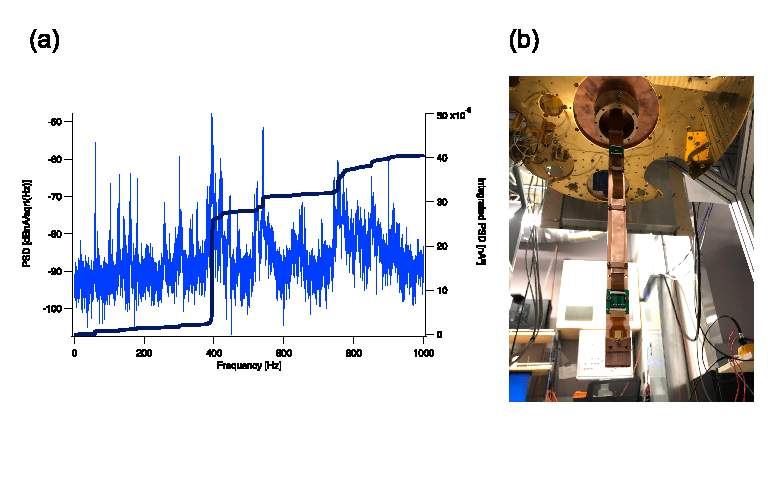
\includegraphics{figures/pdfs/noise.eps}}
\caption{In (a) a current \ac{PSD} and its integral for an open line are plotted indicating an open line noise of about 200 fA/$\sqrt{\textnormal{Hz}}$ in the 0 $\to$ 1 kHz bandwidth. Notably, the majority of the remaining noise can be attributed to a contribution at 400 Hz which we attribute to a vibrational resonance in our wiring. In (b), the coldfinger design utilized for this low noise setup is imaged. Flat flexible cables are used to connect the wiring to a set of RC filters on the face of the MC plate (top of picture). These cables are spray-coated in a thin layer of graphite which limits vibrations from inducing triboelectric noise in the cables.}
\label{fig:noise}       
\end{figure}

As a consequence of the difficulty of limiting triboelectric noise, a number of iterations of wiring were developed with the current iteration shown in Fig.~\ref{fig:noise} (b). Twisted pair Ph-Br unshielded wiring was used from the top of the fridge to the \ac{MC} plate (shown in the top of Fig.~\ref{fig:noise} (b)). This wiring was hand-soldered to a 3-pole RC filter with $f_{char} \approx 60$ kHz. The stages in the filter are 500 Ohm, 2 x 47 pF, 500 Ohm, 2 x 220 pF, and 500 Ohm, 2 x 820 pF. Grounding for this RC filter is defined at the top of the fridge through a separate line. From this filter to the base of the coldfinger a narrow flat flexible kapton + BeCu conductor cable is utilized. This flat flexible cable is coated in a thin layer of graphite to conduct any charge developing from triboelectric effects away. It is then clamped to the coldfinger to limit vibrational noise. 


\chapter{Device Fabrication}

To fabricate the devices referred to in this thesis and previous iterations of similar devices, a number of nano-fabrication recipes were developed and iterated upon. In this section, these processes are described and recipes used are laid out. 

\section{Summary}
\label{sec:summary}

There are two key features to devices built on GaAs/AlGaAs \ac{2DEG}s -- ohmic contact to the \ac{2DEG} and gating structures. In overview, devices used for this project use a thin film of Al$_2$O$_3$ to electrically isolate top-gates fabricated from Au/Pd. Ohmic contacts are made using annealed Ni/Au/Ge. In Fig.~\ref{fig:fab}, a number of the key steps in these processes are illustrated. 

The general process of preparation of a sample goes as follows:
\begin{enumerate}
	\item Gallium removal from back of wafers.
	\item Ohmic contact: lithography, evaporation, annealing.
	\item Mesa etching: lithography, H$_2$S0$_4$ etching.
	\item Atomic layer deposition: Al$_2$O$_3$.
	\item Gating (2 steps): lithography, evaporation.
\end{enumerate}

\begin{figure}[h]
\centering
\resizebox{1\textwidth}{!}{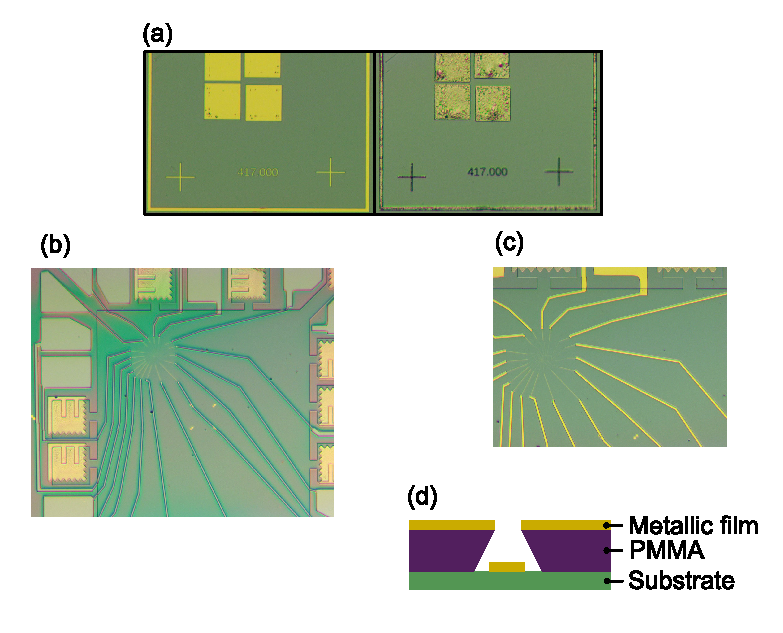
\includegraphics{figures/pdfs/fab_basics.eps}}
\caption{In (a), a sample chip is shown (optical image) before (L) and after (R) annealing. Notably, the process of annealing melts the metals that were evaporated onto the surface of the chip, forming an alloy. The change in surface quality of the metal between the two images shows that this process has occurred. In (b) and (c) a sample pair of optical images show a sample with resist having already been written (b) and this same chip post evaporation (c). In (d), a schematic side view of the lithography process is shown. PMMA forms concave side walls preventing the metallic film from making contact with the substrate, except in areas defined by an electron beam. After a state like that shown in (d) is reached, Acetone can be used to ``liftoff" the unneeded metallic film by dissolving the PMMA on which the metallic film is resting.}
\label{fig:fab}       
\end{figure}

\section{Recipes}
\label{sec:recipes}

\subsection{Gallium removal}
This process is described for completeness, however this recipe was not developed, or iterated on, with my help. This is a recipe developed by Dr. Silvia Luescher Folk.
\begin{enumerate}
	\item Cleave a full wafer into a quarter or half wafer. Blow off any dust bunnies from the surface before starting.
	\item Spin a layer of AZ1518 resists at 4000 RPM for 40s.
	\item Bake the resist for 2min at 100C.
	\item Put a clean wipe on a hotplate and set to 50C. Put wafer face down (gallium side up) onto the clean wipe.
	\item Wipe off gallium with q-tips. Keep wiping until it is all gone.
	\item Spin and bake another layer of AZ1518 (4000 RPM 40s and bake 100C 2min).
	\item Etch 2 min in full strength HCl. Quench etch by transferring to DI water.
	\item Rinse well in DI water. Blow-dry.
	\item Squirt down with Acetone to strip resist from the surface and immediately rinse with IPA.
	\item Soak 3min each in Toluene, Acetone, and IPA. Rinse with IPA and blow dry between each solvent. Spray down with DI water and blow-dry.
\end{enumerate}

\subsection{Mesa Etch}

\begin{enumerate}
	\item Solvent clean -- Acetone, IPA. Rinse in DI, blow dry with N$_2$.
	\item Prebake chip for 2 min at 180C
	\item PMMA A4 950K at 4000 rpm for 40s with a 3 min postbake at 180C.
    \item E-beam lithography in Jeol JBX-8100FS 
    \item Develop in IPA:DI, 7:3 40s at 18C, stop develop in DI
	\item O$_2$ plasma etch in Plasma-etch PE-50, 40s
	\item Etch in 30 mL diluted Sulfuric acid (700 Water:3 H$_2$S0$_4$) + 3 mL H$_2$O$_2$ at 18C for an etch rate of about 5nm/s.
	\item Stop etch in DI water. Remaining resist can be removed with Acetone.
\end{enumerate}

\subsection{Ohmic contact}

\textbf{Lithography and Evaporation}: The following steps have been shown to be capable of making usable ohmic contacts of contact resistances of about 1 k$\Omega$, however continued work has been focussed on optimizing the recipe for further use. 
\begin{enumerate}
	\item Solvent clean -- Acetone, IPA, Ultrasound. Rinse in DI, blow dry with N$_2$.
	\item Prebake chip for 2 min at 180C
	\item Spin MMA/PMMA A4 950K bilayer at 4000 rpm for 40s each with a 3 min postbake at 180C after each layer.
	\item E-beam lithography in Jeol JBX-8100FS at a dose of 450 $\mu$C/cm$^2$.
	\item Develop in IPA:DI, 7:3 40s at 18C, stop develop in DI
	\item O$_2$ plasma etch in Plasma-etch PE-50, 15s
	\item Evaporate the following:
		\begin{center}
		\begin{tabular}{ |c|c|c| } 
		\hline
		Metal & Thickness & Rate \\ \hline\hline
		Ni & 5nm & 1.3\r{A}/s \\ 
		Au & 68nm & 1.7\r{A}/s \\ 
		Ge & 68nm & 1\r{A}/s \\ 
		Au & 68nm & 2\r{A}/s \\ 
		Ni & 50nm & 1.6\r{A}/s \\ 
		Au & 50nm & 2.2\r{A}/s \\ 
		\hline
		\end{tabular}
		\captionof{table}{Evaporation for ohmics}\label{tbl:ohmics}
		\end{center}
	\item Liftoff in Acetone at room temperature.
\end{enumerate}

\textbf{Annealing}: The following process was followed on the rapid thermal annealer made ``in-house" for annealing GaAs and other substrates. The basic idea is to use a bulb in a near vacuum (with some amount of forming gas -- H$_2$ + N$_2$) to heat the sample to a high temperature for a limited amount of time. The metal film melts and sinks into the GaAs substrate to make contact with the \ac{2DEG} which is usually 30-200nm below the surface. A sample of a chip before and after annealing can be seen in Fig.~\ref{fig:fab}.
\begin{enumerate}
	\item Pump down should reach lower limit, 0.133 mbar
	\item Set regulator to 2.5 psi (forming gas)
	\item Open Swagelock valve until pressure reads 10mbars
	\item Close speedivalve until pressure reads 200mbar
	\item Turn on bulb to roughly 34\%, it takes about 5-10 minutes
	\item Wait at 350C  for 2min
	\item Go to 450C as fast as you can, hold it there for 40s
	\item Cool below 300C fast by opening the speedivalve on the pump line all the way, and opening the gas flow. 
	\item Cool to 50C, then vent and let cool to room temp
\end{enumerate}

\subsection{Gating}
\textbf{Inner gates}
\begin{enumerate}
	\item Solvent clean -- Acetone, IPA. Rinse in DI, blow dry with N$_2$.
	\item Prebake chip for 3 min at 180C.
    \item PMMA A2 at 4000 rpm for 40s with a 3 min postbake at 180C.
    \item E-beam lithography in Jeol JBX-8100FS
    \item Develop in IPA:DI, 7:3 40s at 18C, stop by directly drying with N2
    \item Evaporate Pd 2nm, 0.8\r{A}/s then Au 12nm, 1\r{A}/s 
    \item Liftoff in Acetone at room temperature.
\end{enumerate}
\textbf{Outer gates and bondpads}
\begin{enumerate}
	\item Solvent clean -- Acetone, IPA. Rinse in DI, blow dry with N$_2$.
	\item Prebake chip for 3 min at 180C.
    \item Spin MMA/PMMA A4 950K bilayer at 4000 rpm for 40s each with a 3 min then 7 min postbake at 180C after each layer.
    \item E-beam lithography in Jeol JBX-8100FS
    \item Develop in IPA:DI, 7:3 40s at 18C, stop in DI
    \item \item O$_2$ plasma etch in Plasma-etch PE-50, 1 min
    \item Evaporate Ti 10nm, 2\r{A}/s then Au 150nm, 4\r{A}/s 
    \item Liftoff in Acetone at room temperature.
\end{enumerate}

\subsection{Disclaimer}
Although a number of working devices were fabricated according to this process, initial fab on the GaAs/AlGaAs \ac{2DEG} used for the final measurements in this thesis was completed before this project began. Christian Olsen's thesis available here: \url{https://www.nbi.ku.dk/english/theses/masters-theses/christian-olsen/Olsen_CH_Master.pd f} describes in detail the exact process used to complete all but the gating of this \ac{2DEG}, which was completed following the recipes above.





